\documentclass[11pt]{article}

\usepackage[utf8]{inputenc}
\usepackage[T1]{fontenc}
\usepackage{lmodern}
\usepackage[a4paper,margin=1in]{geometry}
\usepackage{amsmath,amssymb}
\usepackage{graphicx}
\usepackage{booktabs}
\usepackage{float}
\usepackage{caption}
\usepackage{xcolor}
\usepackage{siunitx}
\usepackage[hidelinks]{hyperref}

\graphicspath{{../figures/}}
\captionsetup{font=small,labelfont=bf}
\sisetup{group-separator={,},group-minimum-digits=4}

\newcommand{\E}{\mathbb{E}}
\newcommand{\eps}{\varepsilon}

\title{\textbf{Discrete Delta Hedging under Black--Scholes}\\[2pt]
\large Convergence, transaction costs, volatility misspecification and model risk}
\author{Dan Allouche}
\date{\today}

\begin{document}
\maketitle

\begin{abstract}
\noindent
We study, by Monte--Carlo simulation, the performance of the discrete-time
delta-hedging strategy for a short option position in the Black--Scholes market.
Using an \emph{exact} geometric-Brownian-motion scheme, a fully vectorised
hedging engine and common random numbers, we quantify how the hedging error
depends on the rebalancing frequency, the drift, transaction costs, the hedging
volatility, and the choice of underlying model. Every statistic is reported with
its Monte--Carlo standard error. We find that (i) the mean hedging error is
exactly zero under the pricing measure, so the object of interest is its
\emph{dispersion}, which collapses as $n^{-1/2}$ (fitted exponent
$-0.468\pm0.009$); (ii) the dispersion \emph{does} depend on the drift, contrary
to a common simplification; (iii) digital options do not obey the $1/\sqrt{n}$
law (exponent $\approx-0.24$); (iv) transaction costs induce a cost/variance
trade-off with an interior optimal frequency, improved by Leland's adjusted
volatility; (v) the hedging error is governed by realised-vs-implied variance
through the gamma-P\&L identity, validated against the engine to three decimals;
and (vi) under stochastic volatility and jumps the Black--Scholes delta hedge
leaves fat-tailed residual risk. All results are reproducible from the
accompanying \texttt{deltahedge} package and its test suite.
\end{abstract}

\section{Framework}

The risky asset follows a geometric Brownian motion and the money-market account
grows at the risk-free rate $r$:
\[
dS_t = \mu S_t\,dt + \sigma S_t\,dW_t,
\qquad
dB_t = r B_t\,dt .
\]
We sell a European option priced $V(t,S_t)$ and hold the self-financing hedge
$\pi_t = \Delta_t S_t + \beta_t B_t$ with $\Delta_t = \partial_S V$. By It\^o's
formula and the Black--Scholes PDE,
$d\pi_t = \Delta_t\,dS_t + \beta_t\,dB_t$, so in \emph{continuous} time the hedge
replicates the payoff exactly, $\pi_T = V(T,S_T)$. In \emph{discrete} time we
rebalance only at $n$ dates $t_k = kT/n$, leaving the hedging error
\[
\eps_n = \pi_n(T) - \text{payoff}.
\]
The drift $\mu$ never enters the hedge --- the engine observes only realised
prices --- and under the pricing measure ($\mu=r$) the discounted self-financing
portfolio is a martingale, so
\[
\boxed{\;\E[\eps_n] = 0 \quad\text{exactly, at every }n.\;}
\]
The mean is therefore \emph{not} the quantity to study; the dispersion of
$\eps_n$ is. This single observation reframes the entire analysis.

\paragraph{Baseline.}
$r=10\%$, $\sigma=20\%$, $S_0=100$, $K=90$, $T=0.25$\,y;
$N=\num{50000}$ Monte--Carlo paths; frequencies
$n\in\{0,1,3,12,84\}$ (and $252$ for the digital). We use the calendar-day
convention (1\,year $=12$ months $=48$ weeks $=336$ days), so $n=84$ is
\emph{calendar}-daily over a quarter; a real trading quarter has $\approx 63$
trading days, a point we keep explicit rather than hide.

\section{Methodology}

Three methodological choices distinguish this study from a textbook exercise.

\begin{enumerate}
\item \textbf{Exact GBM, not Euler.} Paths use the exact log-Euler scheme
$S_{k+1}=S_k\exp\!\big[(\mu-\tfrac12\sigma^2)\,\delta t + \sigma\sqrt{\delta t}\,Z_k\big]$,
which is exact for GBM. The arithmetic Euler--Maruyama scheme injects an
$O(\delta t)$ bias that would masquerade as a ``hedging error'' at coarse $n$;
the exact scheme removes it (and any risk of negative prices).
\item \textbf{Common random numbers.} All frequencies (and all drifts) are driven
by a single fine Brownian motion, aggregated exactly to each coarser grid, so
cross-frequency comparisons are not blurred by Monte--Carlo noise.
\item \textbf{Signal vs.\ noise.} Every estimate is reported with its standard
error $\mathrm{SE}=\mathrm{std}/\sqrt{N}$ and a $95\%$ confidence interval. A
number is only called ``an effect'' once it is statistically resolved.
\end{enumerate}

\section{Convergence of the call hedge ($\mu=r$)}

Table~\ref{tab:call} reports the hedging error by frequency. The mean is
statistically indistinguishable from zero everywhere (every $p$-value is large,
every $95\%$ CI contains $0$), exactly as the martingale property predicts. The
real, resolved effect is the collapse of the standard deviation, from
$9.59$ (no hedge) to $0.21$ (calendar-daily): a $\sim 98\%$ reduction.

\begin{table}[H]
\centering
\caption{Call hedging error, $N=\num{50000}$, common random numbers across $n$.
The mean is consistent with zero at every frequency; the dispersion is the signal.}
\label{tab:call}
\begin{tabular}{rlrrcrr}
\toprule
$n$ & frequency & mean & SE & $95\%$ CI & std & $p(\text{mean}=0)$ \\
\midrule
0  & No hedging      & $-0.0710$ & 0.0429 & $[-0.155,\,+0.013]$ & 9.5853 & 0.10 \\
1  & Single (static) & $-0.0027$ & 0.0066 & $[-0.016,\,+0.010]$ & 1.4742 & 0.68 \\
3  & Monthly         & $-0.0028$ & 0.0044 & $[-0.011,\,+0.006]$ & 0.9762 & 0.52 \\
12 & Weekly          & $-0.0016$ & 0.0023 & $[-0.006,\,+0.003]$ & 0.5247 & 0.49 \\
84 & Calendar-daily  & $+0.0004$ & 0.0009 & $[-0.001,\,+0.002]$ & 0.2058 & 0.66 \\
\bottomrule
\end{tabular}
\end{table}

\paragraph{The $1/\sqrt{n}$ law, fitted properly.}
A single ratio $\sigma_{n=1}/\sigma_{n=84}\approx 7.2$ is \emph{not} evidence of
$1/\sqrt{n}$ (the law predicts $\sqrt{84}\approx 9.2$). Fitting
$\log\sigma = a + b\log n$ on $n\ge 3$ --- excluding the static $n=1$, which
performs no intermediate rebalancing and lies outside the asymptotic regime ---
gives
\[
b = -0.468 \pm 0.009 \quad (95\%\ \text{CI }[-0.486,-0.450]),
\]
cleanly consistent with the theoretical $-\tfrac12$. The diagnostic
$\sigma\sqrt{n}$ rises from $1.47$ at $n=1$ to a $\approx1.89$ plateau for
$n\ge3$, which is precisely why $n=1$ must be excluded.

\begin{figure}[H]
\centering
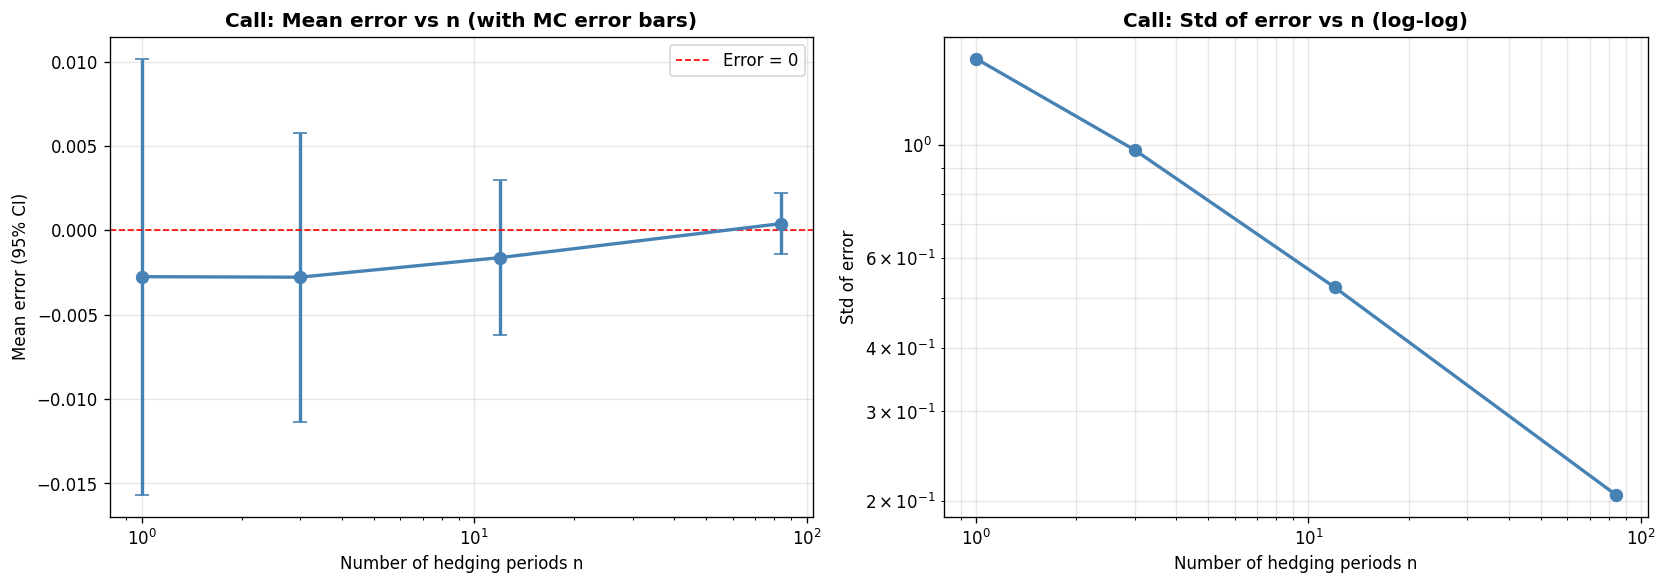
\includegraphics[width=\linewidth]{convergence_call.png}
\caption{Left: mean error with $95\%$ Monte--Carlo error bars (all crossing
zero). Right: standard deviation on a log--log axis --- a clean power law with
slope $\approx-0.47$.}
\end{figure}

\section{Does the drift \texorpdfstring{$\mu$}{mu} matter?}

A common simplification states that the hedging-error variance is controlled by
the rebalancing frequency and not by the drift. This is \emph{false}. Using
common random numbers across $\mu$, the $n=84$ dispersion falls monotonically as
$\mu$ rises (Table~\ref{tab:mu}): a higher drift carries paths deep
in-the-money into the low-gamma region, where there is less gamma-P\&L to
mis-hedge. The mean stays zero throughout --- drift moves the \emph{variance},
not the \emph{bias}.

\begin{table}[H]
\centering
\caption{Standard deviation of the call hedging error at $n=84$ versus drift
$\mu$ (CRN across $\mu$).}
\label{tab:mu}
\begin{tabular}{rrrrrrr}
\toprule
$\mu$ & $-0.10$ & $0.00$ & $0.05$ & $0.10$ & $0.15$ & $0.30$ \\
\midrule
std   & 0.2545 & 0.2325 & 0.2192 & 0.2058 & 0.1941 & 0.1578 \\
\bottomrule
\end{tabular}
\end{table}

\begin{figure}[H]
\centering
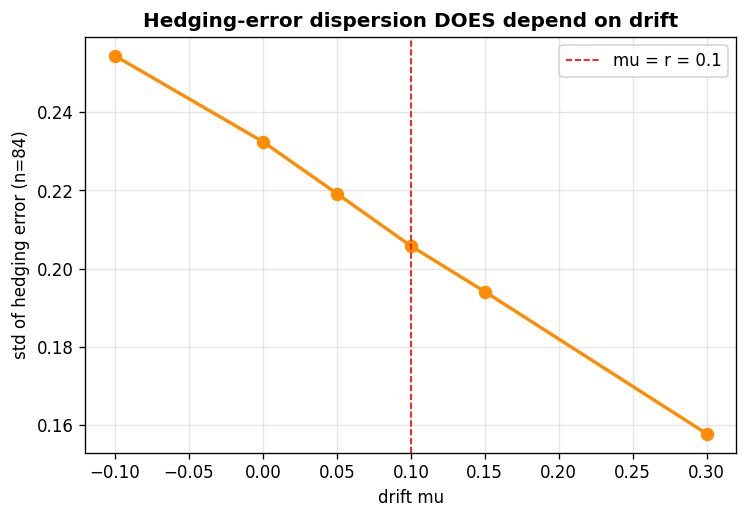
\includegraphics[width=0.72\linewidth]{mu_sensitivity.png}
\caption{Hedging-error dispersion decreases with the drift --- it is not
drift-free.}
\end{figure}

\section{Digital option}

The cash-or-nothing call ($\text{payoff}=\mathbf{1}\{S_T\ge K\}$) is genuinely
harder to hedge. Two findings are real (Table~\ref{tab:digital}): the error
distribution is \emph{bimodal} (clusters at payoff $0$ vs.\ $1$), and the
std-scaling exponent is only $\approx-0.24$ --- the digital error does
\emph{not} obey $1/\sqrt{n}$. Even $n=252$ leaves a std of $\sim0.067$, because
the delta spikes near the strike close to expiry. (By contrast, the original
project's ``non-monotonic mean error'' was pure noise: every $p>0.05$.)

\begin{table}[H]
\centering
\caption{Digital hedging error, $N=\num{50000}$. Means are all consistent with
zero; the dispersion shrinks far more slowly than for the vanilla call.}
\label{tab:digital}
\begin{tabular}{rlrrr}
\toprule
$n$ & frequency & mean & SE & std \\
\midrule
0   & No hedging       & $+0.0001$ & 0.0014 & 0.3066 \\
1   & Single           & $-0.0005$ & 0.0011 & 0.2555 \\
3   & Monthly          & $+0.0000$ & 0.0009 & 0.1990 \\
12  & Weekly           & $+0.0002$ & 0.0006 & 0.1436 \\
84  & Calendar-daily   & $-0.0004$ & 0.0004 & 0.0893 \\
252 & $\sim$4$\times$/trading day & $-0.0004$ & 0.0003 & 0.0673 \\
\bottomrule
\end{tabular}
\end{table}

\begin{figure}[H]
\centering
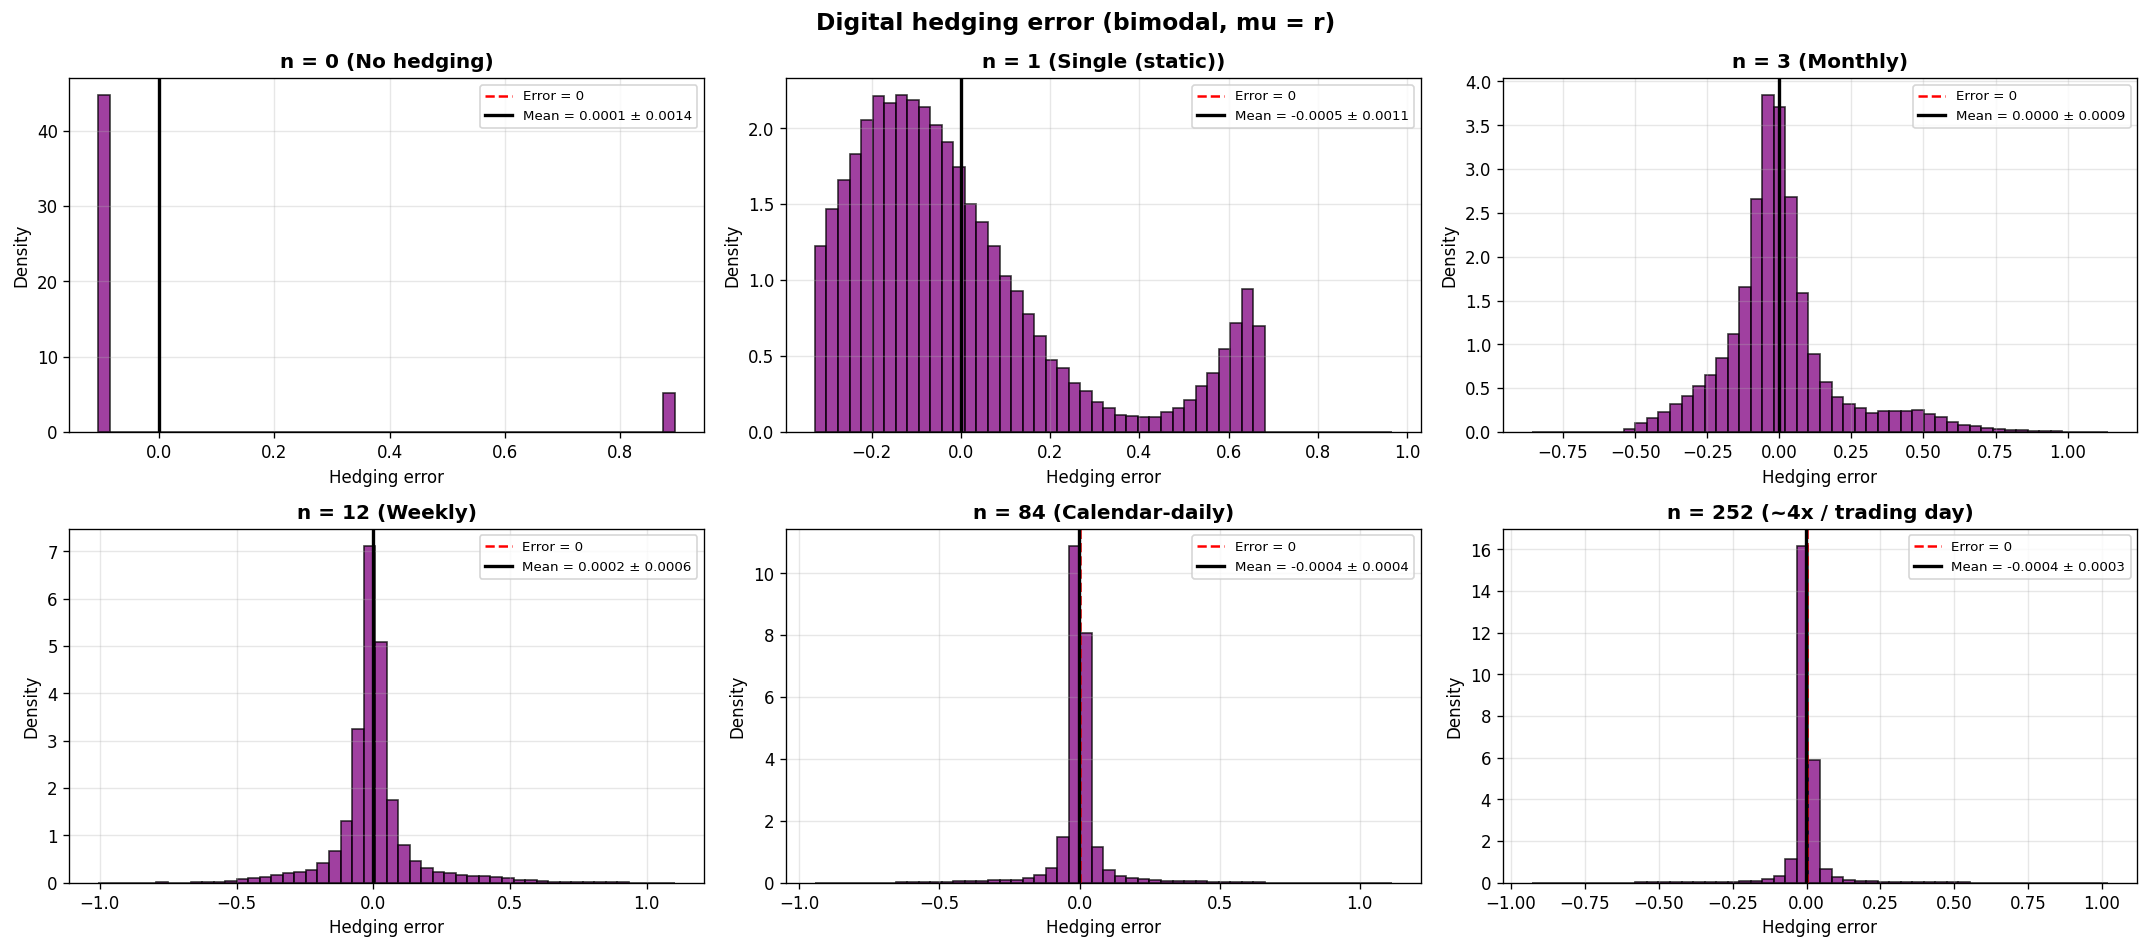
\includegraphics[width=\linewidth]{digital_histograms.png}
\caption{The digital hedging error is bimodal at every frequency, reflecting the
discontinuous payoff.}
\end{figure}

\section{Transaction costs and the Leland adjustment}

With a proportional cost $\kappa$ per unit of underlying traded, more frequent
rebalancing cuts the hedging-error dispersion but raises the expected cost drag.
The two effects trade off, so a tail-risk measure such as the $5\%$ CVaR of the
loss has an \emph{interior optimum}: at $\kappa=0.1\%$ the CVaR-optimal frequency
is $n^\star\approx 168$ (Table~\ref{tab:cost}).

\begin{table}[H]
\centering
\caption{Cost/variance trade-off, $\kappa=0.1\%$. The $5\%$ CVaR of the loss is
minimised at $n^\star=168$.}
\label{tab:cost}
\begin{tabular}{rrrr}
\toprule
$n$ & std(error) & mean cost & $5\%$ CVaR \\
\midrule
3   & 0.9604 & 0.1068 & 3.1145 \\
6   & 0.7210 & 0.1183 & 2.2855 \\
12  & 0.5322 & 0.1329 & 1.6956 \\
21  & 0.4173 & 0.1479 & 1.3599 \\
42  & 0.3082 & 0.1730 & 1.0940 \\
84  & 0.2379 & 0.2078 & 0.9435 \\
\textbf{168} & \textbf{0.2139} & \textbf{0.2581} & \textbf{0.9246} \\
336 & 0.2335 & 0.3276 & 1.0063 \\
\bottomrule
\end{tabular}
\end{table}

\paragraph{Leland (1985).}
Leland's adjusted volatility prices the cost buffer into the hedge,
\[
\sigma_L = \sigma\sqrt{1 + \mathrm{sign}\cdot\sqrt{\tfrac{2}{\pi}}\;
\frac{\kappa}{\sigma\sqrt{\delta t}}}\,.
\]
Hedging the short call at $\sigma_L$ (with $\kappa=0.2\%$, $n=84$) improves the
cost-adjusted P\&L on \emph{both} axes versus the plain $\sigma$ --- higher mean
(less cost drag) and lower dispersion.

\begin{figure}[H]
\centering
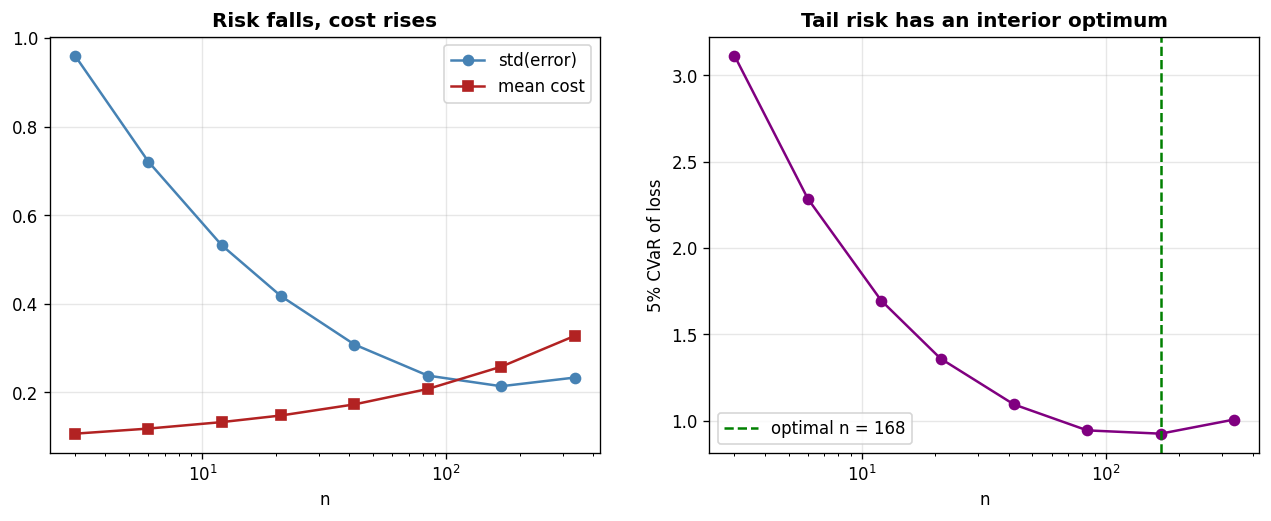
\includegraphics[width=\linewidth]{cost_variance_frontier.png}
\caption{Left: dispersion falls while cost rises with $n$. Right: the $5\%$ CVaR
of the loss has an interior minimum at $n^\star=168$.}
\end{figure}

\begin{figure}[H]
\centering
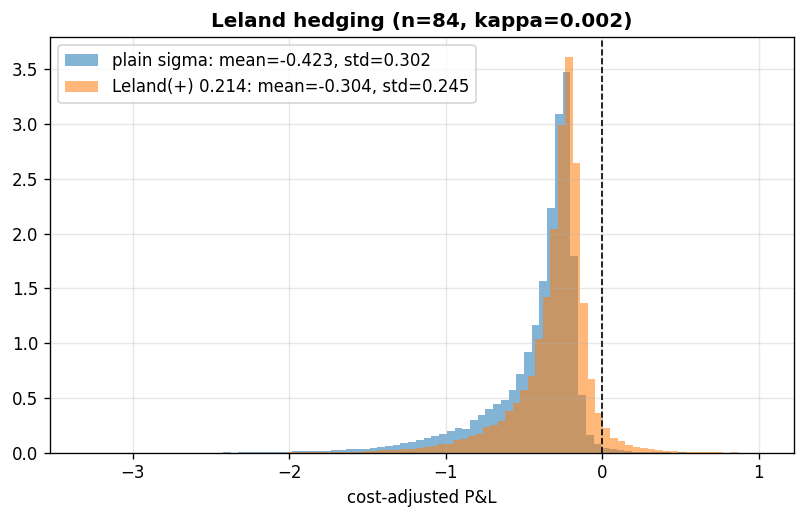
\includegraphics[width=0.78\linewidth]{leland.png}
\caption{Leland's adjusted-volatility hedge shifts the cost-adjusted P\&L
distribution right and tightens it.}
\end{figure}

\section{Volatility misspecification and the gamma-P\&L identity}

This is the central result of option hedging. Hedging at an implied vol
$\sigma_h$ while the asset realises $\sigma_r$, the discrete hedging error of the
short option is, to leading order,
\begin{align*}
\eps \;&\approx\;
-\tfrac12\sum_k \Gamma_k S_k^2
\Big[\big(\tfrac{\Delta S_k}{S_k}\big)^2 - \sigma_h^2\,\delta t\Big] \\[2pt]
&=\;
\underbrace{-\tfrac12\sum_k \Gamma_k S_k^2(\sigma_r^2-\sigma_h^2)\,\delta t}_{\text{deterministic variance mismatch}}
\;+\;
\underbrace{(\text{mean-zero discretisation noise})}_{\sim\,(Z_k^2-1)} ,
\end{align*}
where $\Gamma_k$ is the Black--Scholes gamma at the \emph{hedging} vol. The mean
error is therefore driven by the variance mismatch $\sigma_r^2-\sigma_h^2$, not
the drift --- the ``robustness of Black--Scholes'' result. Empirically the sign
of the mean error tracks $\mathrm{sign}(\sigma_r^2-\sigma_h^2)$ exactly
(Table~\ref{tab:vol}).

\begin{table}[H]
\centering
\caption{Mean call hedging error vs.\ hedging volatility, realised
$\sigma_r=0.20$, $n=84$.}
\label{tab:vol}
\begin{tabular}{rrrrrr}
\toprule
$\sigma_h$ & 0.14 & 0.17 & 0.20 & 0.23 & 0.26 \\
\midrule
mean error & $-0.3481$ & $-0.2102$ & $+0.0004$ & $+0.2735$ & $+0.5972$ \\
\bottomrule
\end{tabular}
\end{table}

The analytic decomposition matches the simulation engine to three decimals: with
$\sigma_r=0.20$, $\sigma_h=0.25$, the engine mean error is $+0.4844$, the
gamma-P\&L sum is $+0.4773$ (correlation $0.994$ path-by-path), and the
deterministic mismatch term alone is $+0.4777$.

\begin{figure}[H]
\centering
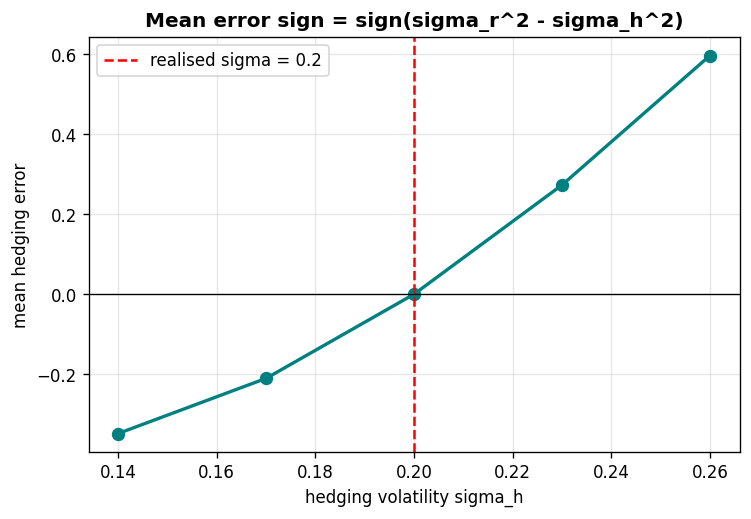
\includegraphics[width=0.72\linewidth]{vol_misspec.png}
\caption{The mean hedging error changes sign exactly at $\sigma_h=\sigma_r$.}
\end{figure}

\section{Greeks-based P\&L attribution}

Desks explain P\&L with a second-order Taylor expansion,
$dV \approx \theta\,dt + \Delta\,dS + \tfrac12\Gamma\,dS^2$. Summed along the path
($n=252$) it reproduces the option's value change to a tiny residual: the
component means are $\theta$-decay $-2.79$, delta $+2.43$, gamma $+0.80$,
giving a predicted $dV=+0.4339$ against an actual $+0.4335$, with residual
standard deviation $0.018$ against an actual-change std of $9.6$ --- the Greeks
explain the P\&L to $\sim 0.2\%$.

\begin{figure}[H]
\centering
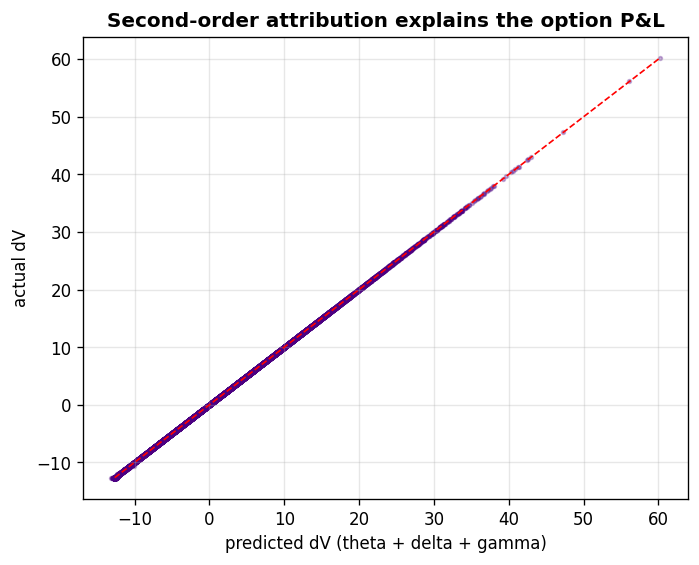
\includegraphics[width=0.6\linewidth]{pnl_attribution.png}
\caption{Predicted (theta $+$ delta $+$ gamma) versus actual value change: the
points lie on the diagonal.}
\end{figure}

\section{Model risk}

Black--Scholes is a model, not reality. Keeping the same BS-delta hedge but
simulating the underlying under \emph{Heston} (stochastic volatility) and
\emph{Merton} (jump diffusion) degrades the hedge sharply (Table~\ref{tab:model}).
Jumps in particular break delta hedging and produce a fat-tailed loss
distribution that no rebalancing frequency can control.

\begin{table}[H]
\centering
\caption{BS-delta hedge ($n=84$) under model misspecification: dispersion and
tail risk of the hedging error.}
\label{tab:model}
\begin{tabular}{lrrrr}
\toprule
underlying model & std & $5\%$ VaR & $5\%$ CVaR & min \\
\midrule
GBM (correct)       & 0.2058 & 0.3252 & 0.5476 & $-2.16$ \\
Heston (stoch.\ vol)& 0.6715 & 1.6490 & 2.4783 & $-7.40$ \\
Merton (jumps)      & 1.4020 & 1.4417 & 5.0280 & $-22.15$ \\
\bottomrule
\end{tabular}
\end{table}

\begin{figure}[H]
\centering
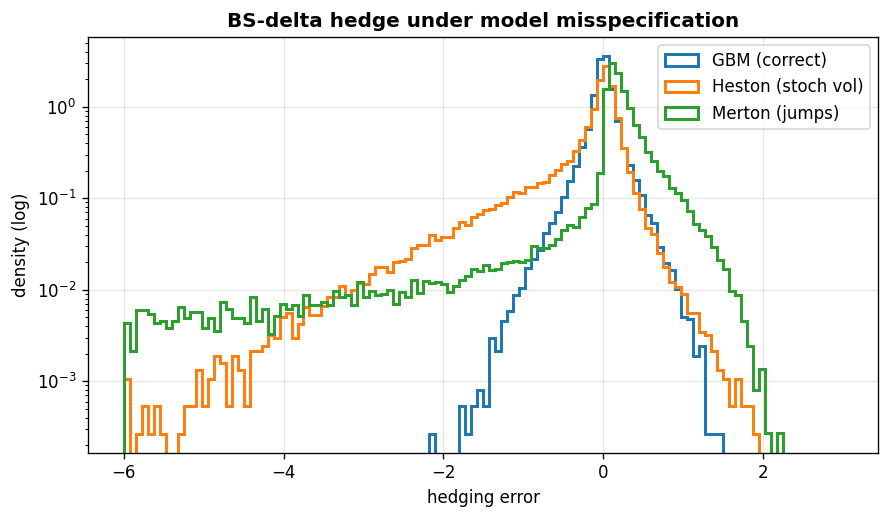
\includegraphics[width=0.82\linewidth]{model_risk.png}
\caption{Hedging-error densities (log scale): the BS hedge is tight under GBM but
develops heavy tails under stochastic volatility and especially jumps.}
\end{figure}

\section{Conclusion}

Discrete delta hedging of a vanilla call converges to perfect replication as the
rebalancing frequency grows, with the error \emph{dispersion} --- not its mean,
which is exactly zero --- scaling as $n^{-1/2}$. That idealised picture is
qualified in every realistic direction studied here: the dispersion depends on
the drift; discontinuous (digital) payoffs converge far more slowly; transaction
costs cap the useful frequency and make Leland's adjustment worthwhile; the
dominant risk is volatility misspecification, governed analytically by the
gamma-P\&L identity; and stochastic volatility or jumps leave fat-tailed residual
risk no frequency can remove. Throughout, reporting Monte--Carlo standard errors
is what separates a resolved effect from sampling noise.

\paragraph{Reproducibility.}
All numbers and figures are produced by the \texttt{deltahedge} package (exact
GBM, $N=\num{50000}$, \texttt{numpy} \texttt{default\_rng} seed
\num{20240614}) and pinned by a \texttt{pytest} regression suite. To reproduce:
\begin{center}
\texttt{pip install -e ".[dev]" \&\& pytest \&\&}\\
\texttt{jupyter nbconvert --to notebook --execute --inplace notebooks/Delta\_Hedging\_Analysis.ipynb}
\end{center}

\end{document}
